%!TEX root = ../dokumentation.tex

\chapter{Auswertung von Messungen mit Hilfe des HRV Evaluation Tools}
In den vorigen Abschnitten wurde bereits ausführlich der Aufbau und die Funktionen des entwickelten Tools erklärt. Nun erfolgt noch eine Beschreibung, wie das Programm in der Praxis tatsächlich genutzt werden kann. Dabei soll vor allem darauf eingegangen werden, welche Verbesserungen und Erleichterungen das HRV Evaluation Tool bei der Analyse von Messungen und der Verwendung von Kubios mit sich bringt. Abschließend soll eine Messung mithilfe des HRV Evaluation Tools analysiert und ausgewertet werden.



\section{Analyse mit Hilfe des  HRV Evaluation Tools und Kubios}
Das HRV Evaluation Tool ist in seiner Entwicklung als Art Hilfestellung für Kubios gedacht. Im Folgenden werden am Beispiel einer Messanalyse die Aspekte beschrieben, in denen sichtbar wird, inwiefern das Evaluation Tool die Nutzung von Kubios vereinfacht.\\

Die Messung, welche analysiert wird hat eine Länge von circa 45 Minuten. Während der gesamten Messung, liegt der Proband ruhig auf einer Liege und betätigt sich nicht körperlich. Zufällig werden während dieses 45 minütigen Messzeitraums ein WLAN Router und eine DECT Basisstation nahe dem Probanden aktiviert, welcher dies allerdings nicht mitbekommt. Die Dauer der elektromagnetischen Belastung beträgt 15 Minuten. Danach werden Router und DECT Basisstation wieder deaktiviert, sodass keine Belastung mehr auf den Probanden einwirkt. Das Belastungsintervall ist dabei Schwerpunkt der Analyse. Dabei soll untersucht werden, ob die elektromagnetische Belastung eine Auswirkung auf die HRV des Probanden hat.

\subsection{Erstellung von Samples}
Die Erstellung der Samples wurde bereits im ersten Kapitel \color{red} 1.3.1 irhgenwie ref \color{black} behandelt. Die zentrale Aussage dabei war, dass das Erstellen von Samples in Kubios einen großen Zeitaufwand erfordert. Um diese Zeit zu sparen, wird zuerst mit dem HRV Evaluation Tool \color{red} die .csv Datei erstellt, welche die gewünschten Samples beinhaltet. \color{black}
Für diese Messung wurde eine Sample Länge von 5 Minuten gewählt. Die Verschiebung zwischen den einzelnen Samples beträgt 1 Minute, sodass jede Minute ein neues Sample beginnt. Die dadurch entstehenden 31 Samples werden beim Laden der Messung in Kubios automatisch erstellt, wodurch viel Zeit eingespart werden konnte.  
\color{red} BILD DAS SAMPLES ZEIGT JA NEIN?. \color{black}
Als nächster Schritt muss die Messung mit ihren Samples aus Kubios als \textit{.mat} Datei exportiert werden, damit sie in das Evaluation Tool geladen werden kann. 

\subsection{Veranschaulichung der Parameter} \label{sec:anschaulich}
Wenn die Messung in das Evaluation Tool geladen wurde, kann zwischen einer Auswahl an Parametern ausgesucht werden. Für den ausgewählten Parameter wird dann ein Wert für jedes Sample berechnet. Diese werden grafisch in einem Diagramm veranschaulicht. Die Darstellung des RMMSD für die Messung ist in Abbildung \ref{fig:rmssd} dargestellt.
\begin{figure}[H]
	\centering
	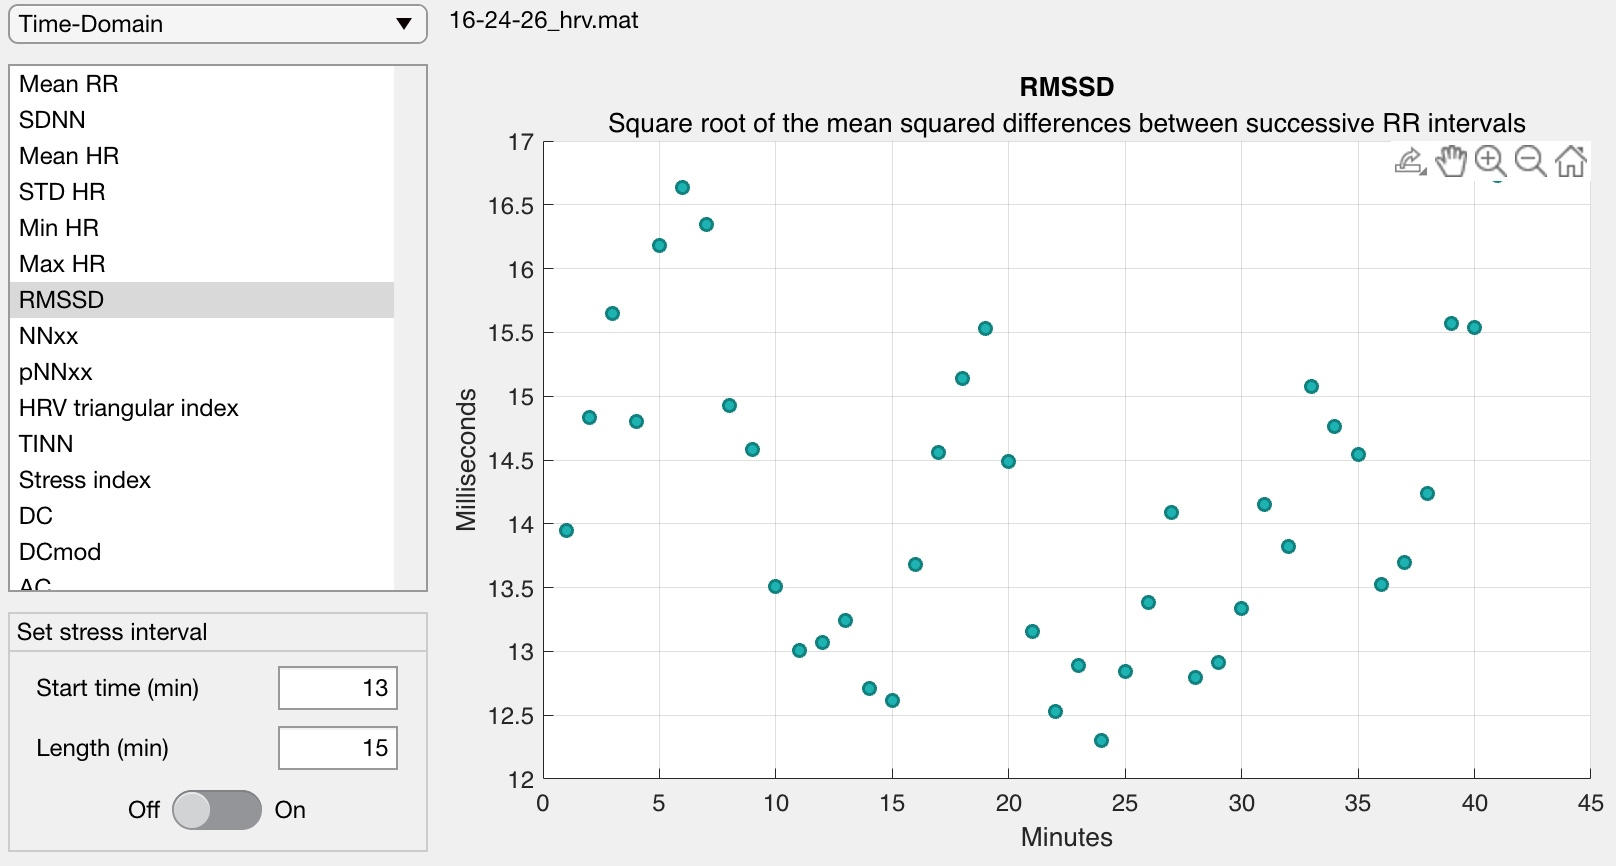
\includegraphics[width=1.0\linewidth]{rmssd}
	\caption{Diagramm des RMSSD }
	\label{fig:rmssd}
\end{figure}
Der RMSSD liegt während der gesamten Messung zwischen 12 und 17ms. Diese Werte sind grundsätzlich eher gering, jedoch nicht so niedrig, dass sie akut auf eine Erkrankung hindeuten. Die Werte deuten lediglich auf eine verminderte kurzzeitige Erholungsfähigkeit des Probanden hin. Auch könnte sich vermuten lassen, dass die Fitness des Probanden nicht optimal ist. Auch ein ungesunden Lebensstil kann Ursache für einen niedrigen RMSSD Wert sein. \\
Dies sind jedoch alles nur Vermutungen, da sich solche Vermutungen nie nur anhand einer Messung bestätigt werden können. Um die aufgestellten Vermutungen beweisen zu können, sind andere Messung außerhalb der HRV nötig. So können verschiedene Sporttests, wie beispielsweise Ausdauertests genutzt werden, um Aussagen über die Fitness treffen zu können.\\
Auffallend sind die hohen Werte zu Beginn und am Ende des Messzeitraums. Dies können ihre Ursache außerhalb der natürlichen Regulierung des autonomen Nervensystems haben. Besonders zu Beginn der Messung kann eine erhöhte Aufregung des Patienten die Werte verfälschen. Auch Messfehler können hier ein Rolle spielen. Deshalb sind Messdaten zu Beginn und am Ende der Messung vorsichtig zu betrachten. Grundsätzlich lässt sich allerdings erkennen, dass der RMSSD zu Beginn und am Ende für diese Messung überdurchschnittlich hoch ist.


\section{Auswertung von Messungen im Bezug auf elektromagnetische Strahlung}
Im Abschnitt \ref{sec:anschaulich} wurde bereits der RMSSD des Probanden über die gesamte Messdauer betrachtet. Nun soll der Einfluss der elektromagnetischen Wellen auf den Probanden genauer untersucht werden. Die Belastungszeitraum war zwischen der 13. und 28. Minuten und kann mit Hilfe des Evaluation Tools farbig in das Diagramm eingezeichnet werden.
\begin{figure}[H]
	\centering
	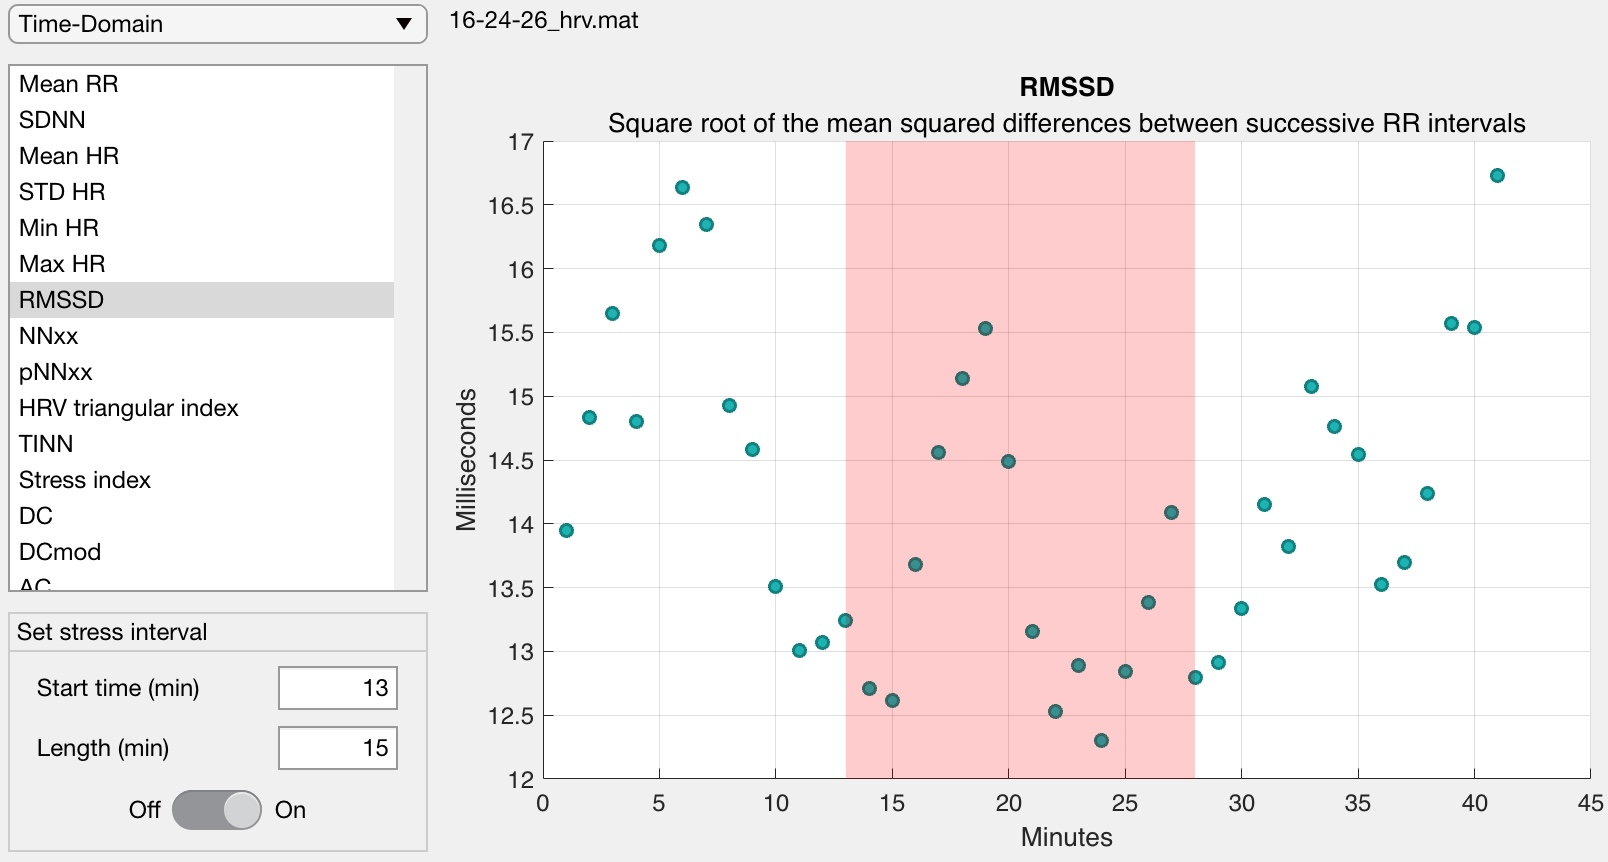
\includegraphics[width=1.0\linewidth]{rmssdbelastung}
	\caption{RMSSD mit eingezeichnetem Belastungsintervall }
	\label{fig:rmssdbelastung}
\end{figure}
Auf den ersten Blick fällt vor allem ein großer Ausschlag des RMSSD nach oben auf. Dieser Ausschlag ist ungefähr in der Mitte des Belastungsintervall. Nach diesem Ausschlag fällt der RMSSD sehr stark ab, sodass gegen Ende der Belastung mit nur knapp über 12 ms der geringste Wert der gesamtem Messung aufgezeichnet wurde. Auch zu Beginn des Belastungsintervalls sind die Werte des RMSSD gering. \\
Bei Einordnung der Belastung in die gesamte Messdauer fällt auf, dass mit Ausnahme der kurzzeitigen hohen Messwerte in der Mitte des Belastungsintervall, der RMSSD während der Belastung unterdurchschnittlich gering ist. Hier lässt sich die These aufstellen, dass die elektromagnetische Strahlung eine negative Auswirkung auf den RMSSD und der damit zusammenhängenden kurzzeitigen Erholungsfähigkeit des Probanden hat. Um diese Theorie weiter zu untersuchen könnte als nächstes eine längere Messung durchgeführt werden. Auch die Untersuchung von Messungen mit mehreren Belastungsintervallen würden weiteren Erkenntnisgewinn bringen. \\
Eine weitere Möglichkeit ist es, sich die gemessenen NN-Intervalle an sich anzuschauen. Oft ergibt sich bereits am Verlauf der NN-Intervalle weitere Erkenntnis, wie in Abbildung \ref{fig:meanrr} dargestellt
\begin{figure}[H]
	\centering
	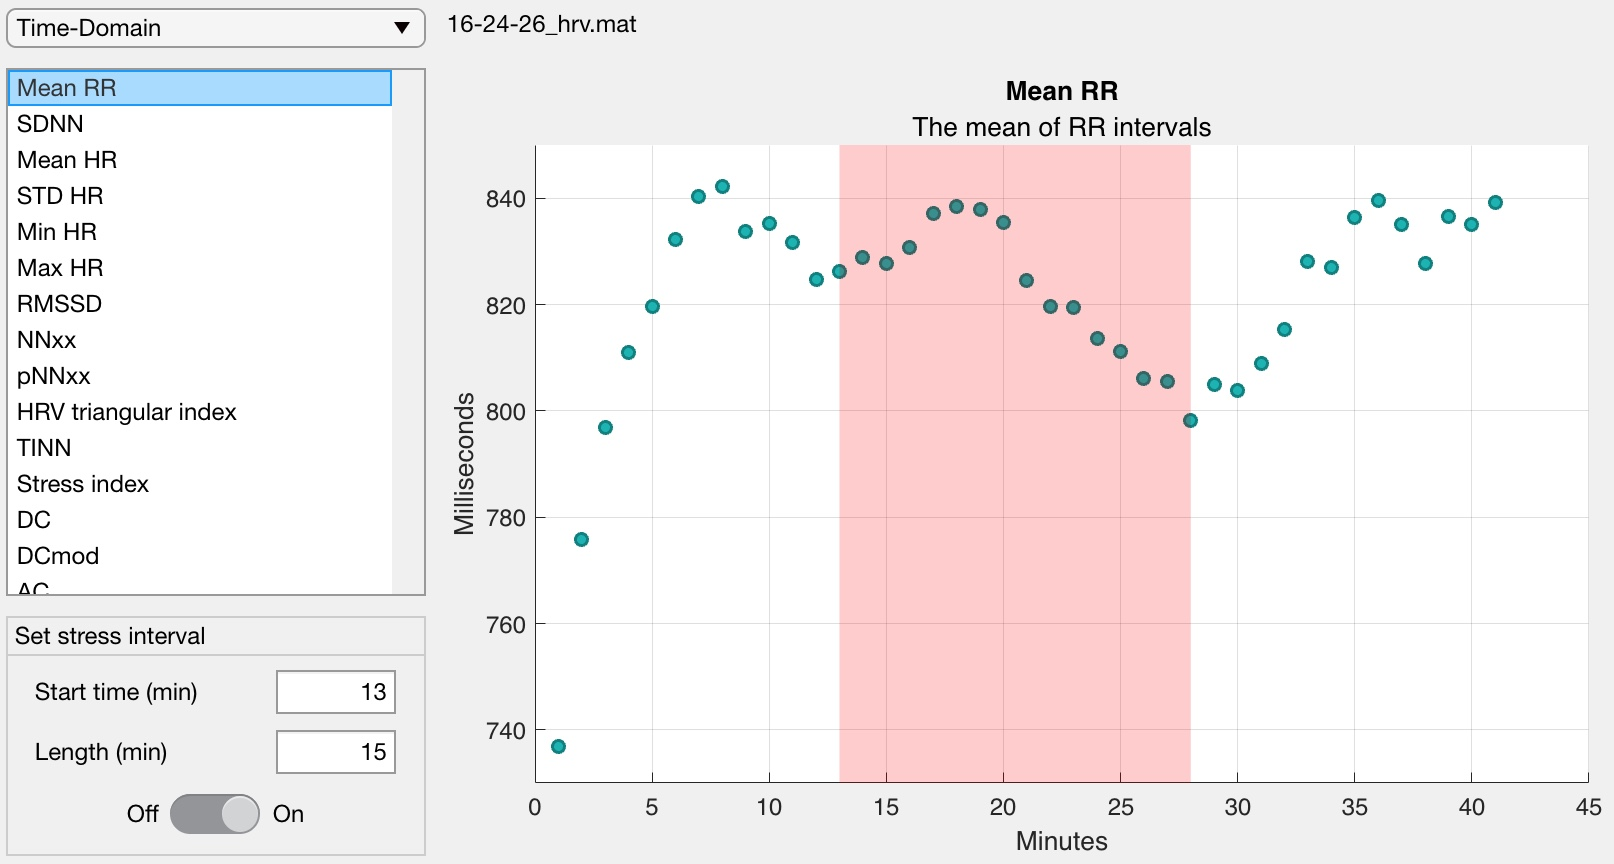
\includegraphics[width=1.0\linewidth]{meanrr}
	\caption{RMSSD mit eingezeichnetem Belastungsintervall }
	\label{fig:meanrr}
\end{figure}

Die Intervalldauer ist zu Beginn der Messung sehr niedrig, steigt dann aber steil an. Dieser abrupte Anstieg deutet stark auf einen Messfehler hin, da die Starke Änderung der NN-Intervalldauer in einem so kurzen Zeitabschnitt ohne plötzliches Ereignis von Außen eher unwahrscheinlich ist. Auch findet sich im weiteren Verlauf der Messung keine so starke Änderung wieder.\\

Zu Beginn des Belastungsintervalls lässt sich wie beim RMSSD eine Verbesserung feststellen. Danach ist allerdings ein monotone Abnahme der HRV bis zum Ende der Belastung sichtbar. So wurde genau zu Ende des Belastungsintervall der geringste Wert mit knapp 800ms gemessen. Nach der Belastung steigt die Dauer der NN-Intervalle wieder an und erreicht ungefähr das gleiche Niveau wie vor der Belastung. \\
Die Betrachtung der durchschnittlichen NN-Intervalldauer stärkt die These, dass elektromagnetische Strahlung sich negativ auf die Herzratenvariabilität des Probanden auswirkt. Besonders die fast durchgängige monotone Verschlechterung der HRV während der Belastung ist auffällig. Um das Verhalten der HRV während elektromagnetischer Strahlung weiter zu untersuchen, ist das Berechnen weiterer HRV Parameter sinnvoll. So kann beispielsweise der SDNN, ein Parameter für die langzeitige Erholungsfähigkeit des Körpers, weitere Informationen liefern. Dieser ist in Abbildung \ref{fig:sdnn} dargestellt.
\begin{figure}[H]
	\centering
	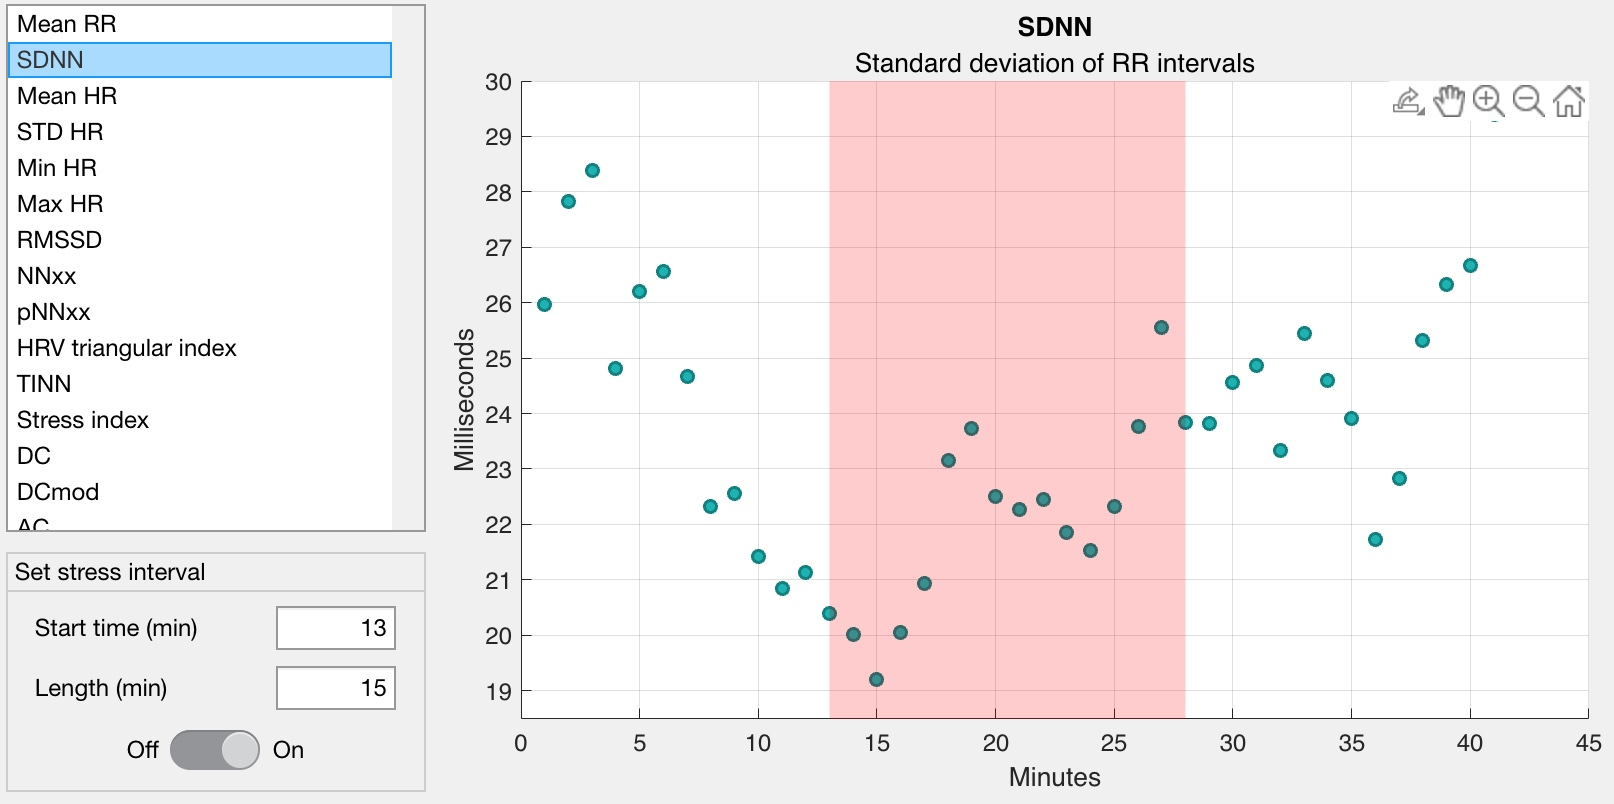
\includegraphics[width=1.0\linewidth]{sdnn}
	\caption{RMSSD mit eingezeichnetem Belastungsintervall }
	\label{fig:sdnn}
\end{figure}


Der Wert des SDNN startet zu Beginn der Messung bereits sehr hoch, sodass nach ungefähr 3 Minuten der höchste Wert mit knapp über 28 ms gemessen wurde. Danach sinkt der Wert konstant bis zum Start des Belastungsintervall. Kurz nach Start der Belastung lässt sich eine fast konstante Verbesserung des SDNN bis zum Ende der Messung erkennen. \\
Anhand es SDNN lassen sich keine negativen Auswirkungen von elektromagnetischen Wellen auf den Körper erkennen. Es kann sogar fast gegenteilig argumentiert werden. Ab Beginn der Belastung steigt der Wert des SDNN kontinuierlich an. Auch das Beenden der Belastung hatte keine ersichtliche Auswirkung auf den SDNN. 

Die bisherigen Parameter wurden alle an der gleichen Messung berechnet. Um weiteren Aufschluss auf die Auswirkung elektromagnetischer Strahlung zu erhalten müssen mehrere Messungen betrachtet werden. Der RMSSD 

